\documentclass[11pt,a4paper]{article}
\usepackage[utf8]{inputenc}
\usepackage[T1]{fontenc}
\usepackage[polish]{babel}
\usepackage{amsmath}
\usepackage{amsfonts}
\usepackage{amssymb}
\usepackage{graphicx}
\usepackage{booktabs}
\usepackage{hyperref}
\usepackage{geometry}
\usepackage{float}
\usepackage{caption}

\geometry{margin=2.5cm}

\title{\textbf{Zastosowanie Uczenia Maszynowego w Adaptacji Łącza Radiowego dla Systemów 5G NR}}
\author{Filip Ferenc}
\date{\today}

\begin{document}

\maketitle

\begin{abstract}
Raport przedstawia wyniki prac nad systemem adaptacji łącza (Link Adaptation) dla stacji bazowych 5G NR z wykorzystaniem uczenia maszynowego. Głównym celem było zastąpienie heurystycznego algorytmu OLLA modelem przewidującym optymalny schemat modulacji i kodowania (MCS), spełniającym rygorystyczne wymagania czasowe warstwy MAC (czas inferencji poniżej 1 ms). Zastosowano regresję porządkową opartą na Gradient Boosting Machine (GBM) z ograniczeniami monotonicznymi, a następnie skompresowano model za pomocą destylacji wiedzy do postaci prostego drzewa decyzyjnego. Wyniki symulacji oraz testów na żywo w środowisku srsRAN potwierdzają stabilność i wysoką wydajność zaproponowanego hybrydowego podejścia (GBM + OLLA).
\end{abstract}

\section{Wstęp}

W sieciach komórkowych 5G stacja bazowa (gNB) odpowiada za dynamiczny dobór parametrów transmisji dla każdego użytkownika (UE). Kluczowym zadaniem jest określenie optymalnego schematu modulacji i kodowania (MCS). Wybór zbyt niskiego wskaźnika MCS ogranicza przepustowość, natomiast zbyt wysoki prowadzi do błędów transmisji i konieczności retransmisji pakietów (wzrost opóźnień). 

Tradycyjne podejście opiera się na raportach jakości kanału (CQI) wysyłanych przez UE, które stacja bazowa mapuje na MCS korzystając z gotowych tabel (Look-Up Tables) oraz koryguje za pomocą pętli sprzężenia zwrotnego OLLA (Outer Loop Link Adaptation). Rozwiązanie to słabo radzi sobie w wysoce dynamicznych środowiskach (np. szybki ruch pojazdów, nagłe interferencje). Celem projektu było zaprojektowanie inteligentnego algorytmu selekcji MCS, który na podstawie bieżących metryk sygnałowych zmaksymalizuje przepustowość, utrzymując jednocześnie współczynnik błędu bloku (BLER) poniżej progu 10\%.

\section{Wybór Architektury Modelu ML}

Dobór odpowiedniej architektury modelu uczenia maszynowego podyktowany był specyfiką warstwy MAC (Medium Access Control) oraz fizyką propagacji fal radiowych. 

\subsection{Regresja Porządkowa vs Klasyfikacja}
Indeksy MCS (0--28) posiadają naturalny porządek. Traktowanie ich jako niezależnych klas w standardowym klasyfikatorze sieci neuronowej jest błędem, ponieważ kara za pomyłkę pomiędzy MCS 14 a 15 powinna być mniejsza niż pomiędzy MCS 14 a 5. Co więcej, przeszacowanie (zbyt wysoki MCS) skutkuje utratą pakietu, podczas gdy niedoszacowanie jedynie nieznacznym spadkiem przepustowości. Z tego powodu sformułowano problem jako \textbf{regresję porządkową (ordinal regression)} z asymetryczną funkcją kosztu, która silniej karze przeszacowanie.

\subsection{Gradient Boosting i Ograniczenia Monotoniczne}
Standardowe głębokie sieci neuronowe (DNN) nie gwarantują zachowania zasad fizyki -- mogą na przykład zaproponować niższy MCS dla wyższego stosunku sygnału do szumu (SINR). Aby wyeliminować takie anomalie, wybrano modele oparte na drzewach decyzyjnych (Gradient Boosted Machines -- GBM), które pozwalają na nałożenie twardych ograniczeń monotonicznych. Gwarantuje to, że wzrost jakości sygnału lub spadek prędkości UE nigdy nie doprowadzi do obniżenia wybranego MCS.

\subsection{Destylacja Wiedzy dla Czasu Rzeczywistego}
Scheduler warstwy MAC w sieciach 5G działa z precyzją rzędu mikrosekund (budżet czasowy rzędu 1 ms na slot). Ewaluacja złożonego modelu GBM złożonego z setek drzew zajmuje zbyt dużo czasu (ok. 10 ms). Zastosowano więc technikę \textbf{destylacji wiedzy}. Rozbudowany model GBM posłużył jako ``nauczyciel'' dla pojedynczego, stosunkowo płytkiego drzewa decyzyjnego (maksymalna głębokość 10). Takie drzewo kompiluje się do kaskady prostych instrukcji warunkowych w języku C++, co pozwala na inferencję bez dynamicznej alokacji pamięci.

\subsection{Hybrydowe Podejście GBM + OLLA}
Samo drzewo decyzyjne operuje w pętli otwartej i nie jest w stanie zareagować na nieprzewidziane anomalie kanału. Z tego powodu model ML zintegrowano z klasycznym mechanizmem OLLA. Drzewo wyznacza stabilny punkt startowy MCS na podstawie warunków radiowych, a OLLA delikatnie go koryguje na podstawie spływających potwierdzeń (ACK/NACK). Podejście to niweluje niestabilność, z którą borykały się testowane wcześniej sieci neuronowe złączone z OLLA.

\section{Metodologia i Środowisko Badawcze}

\subsection{Generacja Danych (NVIDIA Sionna)}
Model wymagał bogatego zestawu danych odzwierciedlającego fizykę propagacji fal. Za pomocą symulatora \textbf{NVIDIA Sionna} wygenerowano zbiór ponad 2,2 miliona pakietów. W symulacjach uwzględniono:
\begin{itemize}
    \item Modele kanałów 3GPP (TDL-A dla środowisk biurowych, TDL-B/C dla miejskich, CDL-D).
    \item Efekt Dopplera odpowiadający prędkościom UE od 3 km/h do 120 km/h.
    \item Konfiguracje antenowe SISO oraz MIMO 2x2 w pasmach sub-6 GHz oraz mmWave.
\end{itemize}

\subsection{Cechy Wejściowe (Features) i Ograniczenia}
Model podejmuje decyzje na podstawie 6 parametrów. Część z nich (np. SINR, konfiguracja antenowa) jest bezpośrednio dostępna w stacji bazowej. Należy jednak zaznaczyć obiektywne ograniczenia obecnej wersji algorytmu: prędkość UE oraz profil opóźnień kanału (TDL) nie są trywialne do zmierzenia w czasie rzeczywistym. W prototypie parametry te są wprost dostarczane do algorytmu, lecz w wersji produkcyjnej wymagałyby one wdrożenia dodatkowych estymatorów (np. estymacji rozrzutu Dopplera z sygnałów SRS).

\section{Wyniki Eksperymentalne}

Ewaluację podzielono na analizę offline, symulację zamkniętej pętli oraz wdrożenie w stosie srsRAN.

\subsection{Analiza Offline (Porównanie Metod)}
Przeprowadzono analizę 8 różnych strategii adaptacji łącza (10 powtórzeń, 95\% przedziały ufności). Wyniki (Tabela \ref{tab:offline}) wskazują, że zaproponowany model Ordinal GBM z ograniczeniami osiąga przepustowość zbliżoną do modeli opartych na sieciach neuronowych (DNN), zapewniając przy tym znacznie wyższą stabilność i pozwalając na łatwy eksport do kodu C++.

\begin{figure}[H]
    \centering
    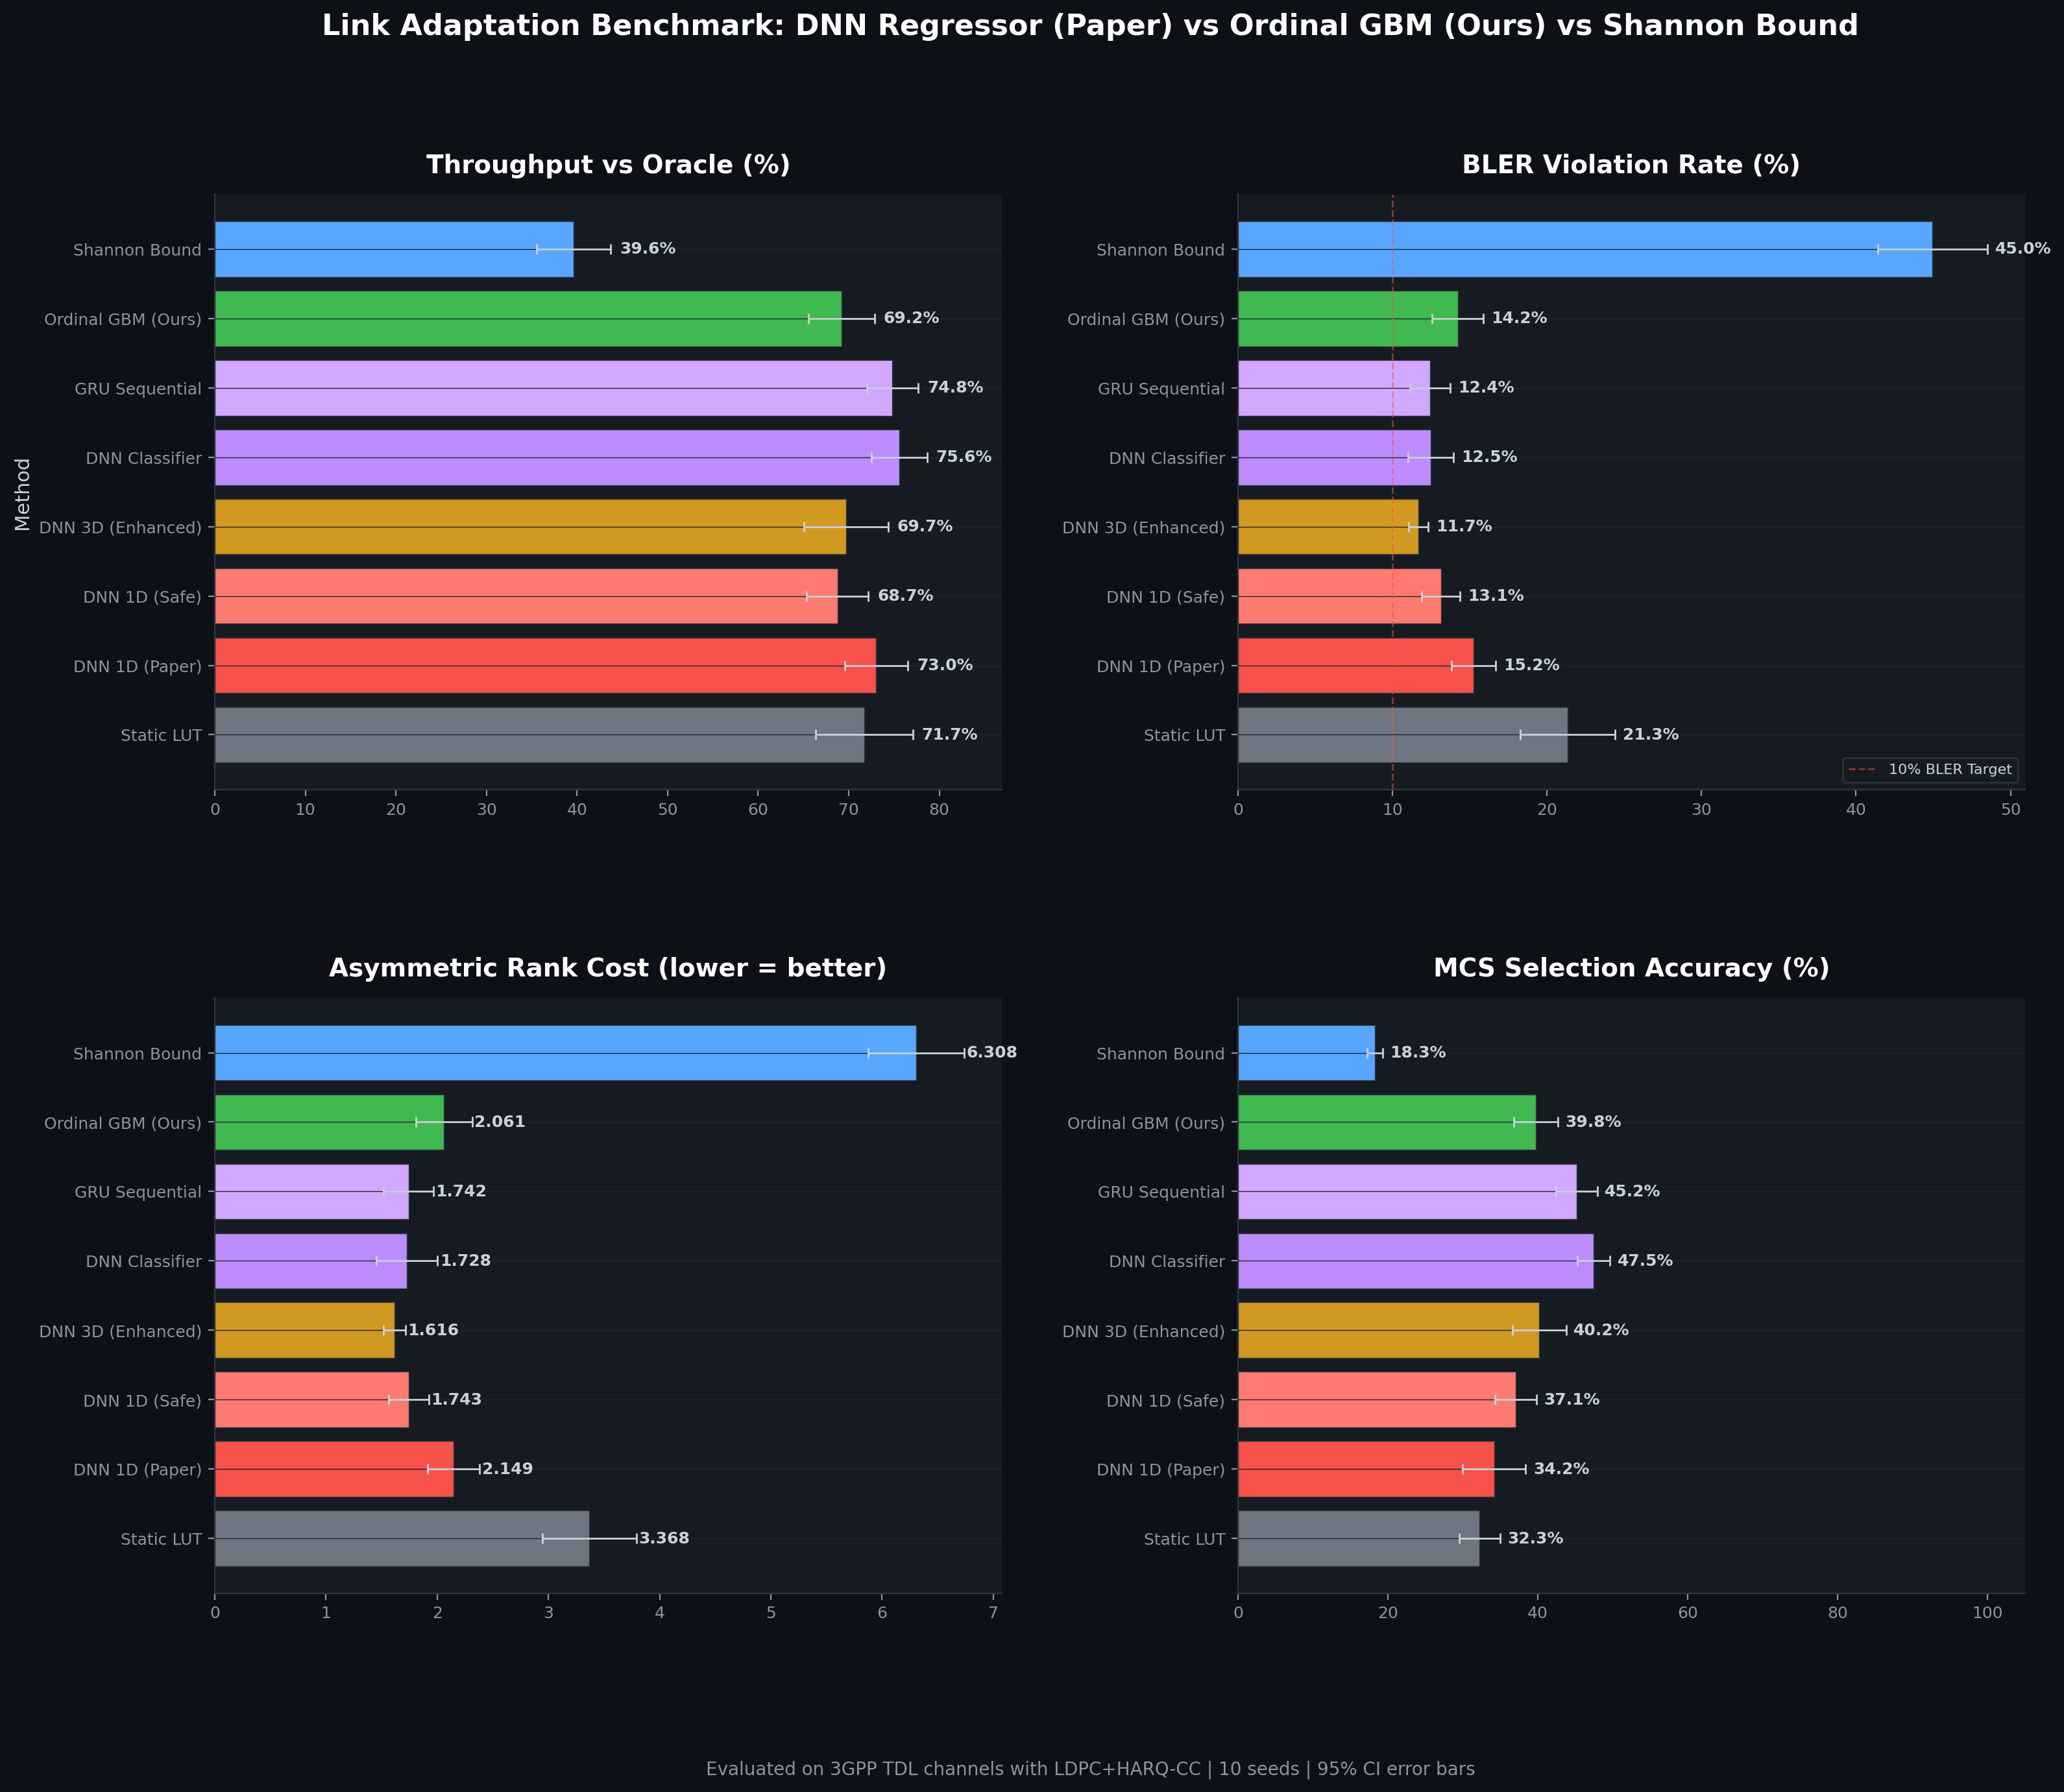
\includegraphics[width=0.9\textwidth]{results/la_benchmark_comparison.png}
    \caption{Porównanie przepustowości i naruszeń BLER dla różnych metod adaptacji łącza.}
    \label{fig:offline_benchmark}
\end{figure}

\begin{table}[H]
\centering
\begin{tabular}{lcc}
\toprule
\textbf{Metoda} & \textbf{Przepustowość względem ideału (Oracle)} & \textbf{Naruszenia BLER ($>10\%$)} \\
\midrule
Static LUT & 71.7\% & 21.3\% \\
DNN 1D (literaturowy) & 73.0\% & 15.2\% \\
\textbf{Ordinal GBM (Nasz)} & \textbf{69.2\%} & \textbf{14.2\%} \\
GRU Sequential & 74.8\% & 12.4\% \\
\bottomrule
\end{tabular}
\caption{Wybrane wyniki ewaluacji offline.}
\label{tab:offline}
\end{table}

Ponadto zbadano stabilność modelu względem różnych profili kanałów radiowych (CDL-D, TDL-A, TDL-C). Model wykazuje konsekwentną skuteczność w każdym ze środowisk.

\begin{figure}[H]
    \centering
    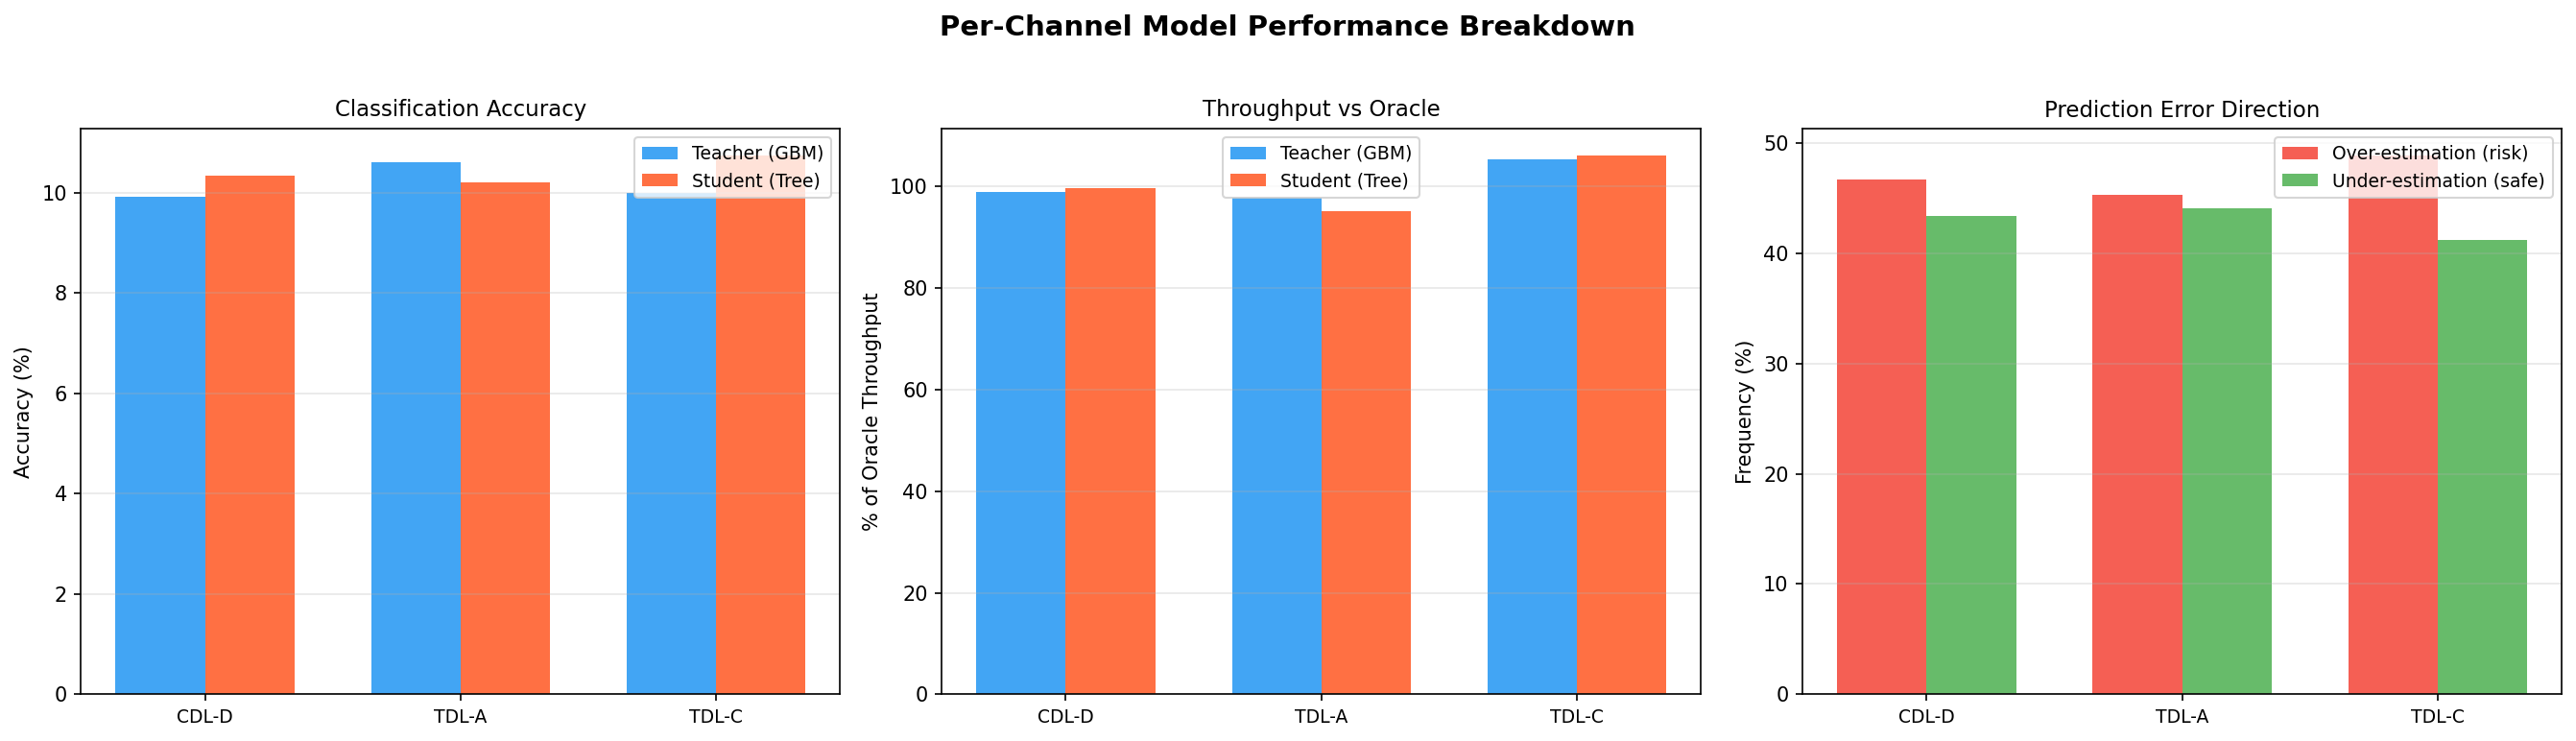
\includegraphics[width=0.7\textwidth]{results/channel_breakdown.png}
    \caption{Wydajność modelu w zależności od profilu propagacyjnego kanału.}
    \label{fig:channel_breakdown}
\end{figure}

\subsection{Destylacja i Zależność od SNR}
Pojedyncze drzewo decyzyjne zostało wygenerowane na podstawie zespołu GBM. Analiza jakości destylacji wykazała ok. 68\% całkowitej zgodności oraz ponad 70\% w przedziale odchylenia o $\pm1$ krok MCS. Zostało to udokumentowane w postaci macierzy pomyłek (ang. confusion matrix). Zbadano także zachowanie schodkowe modelu względem narastającego SINR.

\begin{figure}[H]
    \centering
    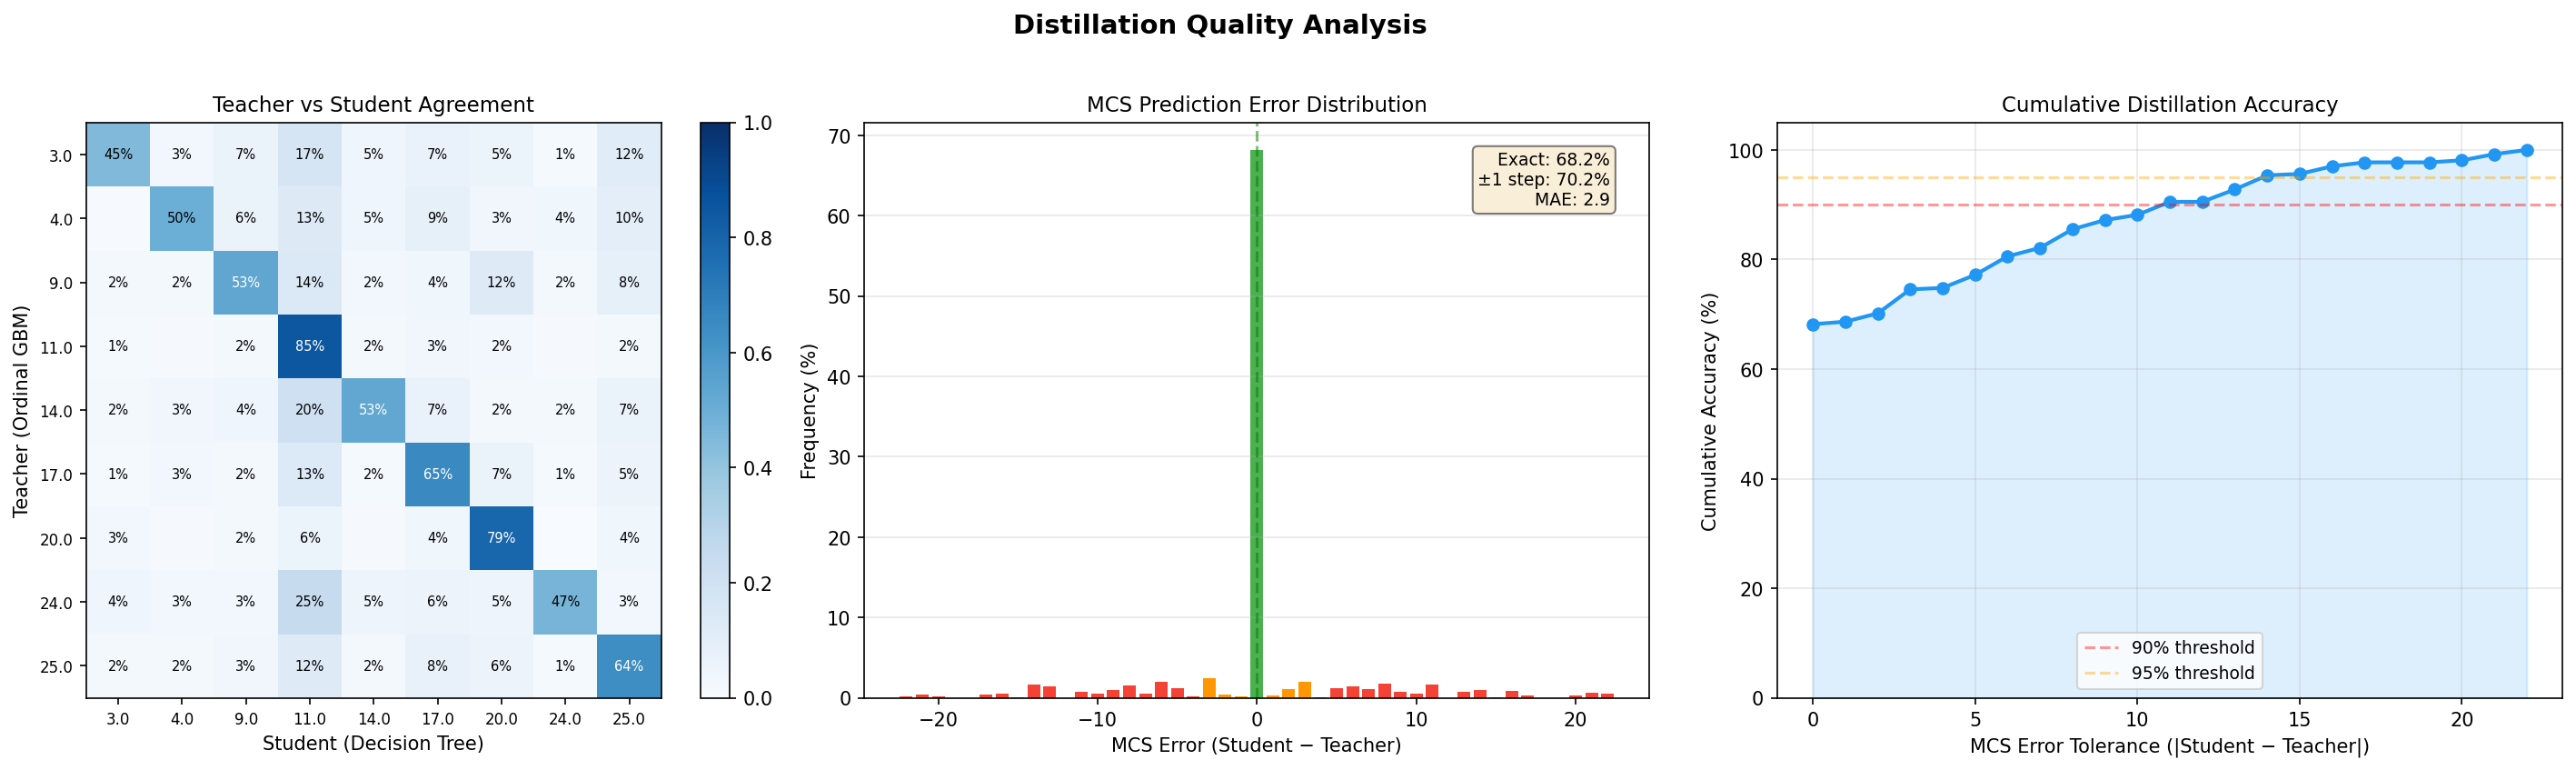
\includegraphics[width=0.48\textwidth]{results/distillation_analysis.png}
    \hfill
    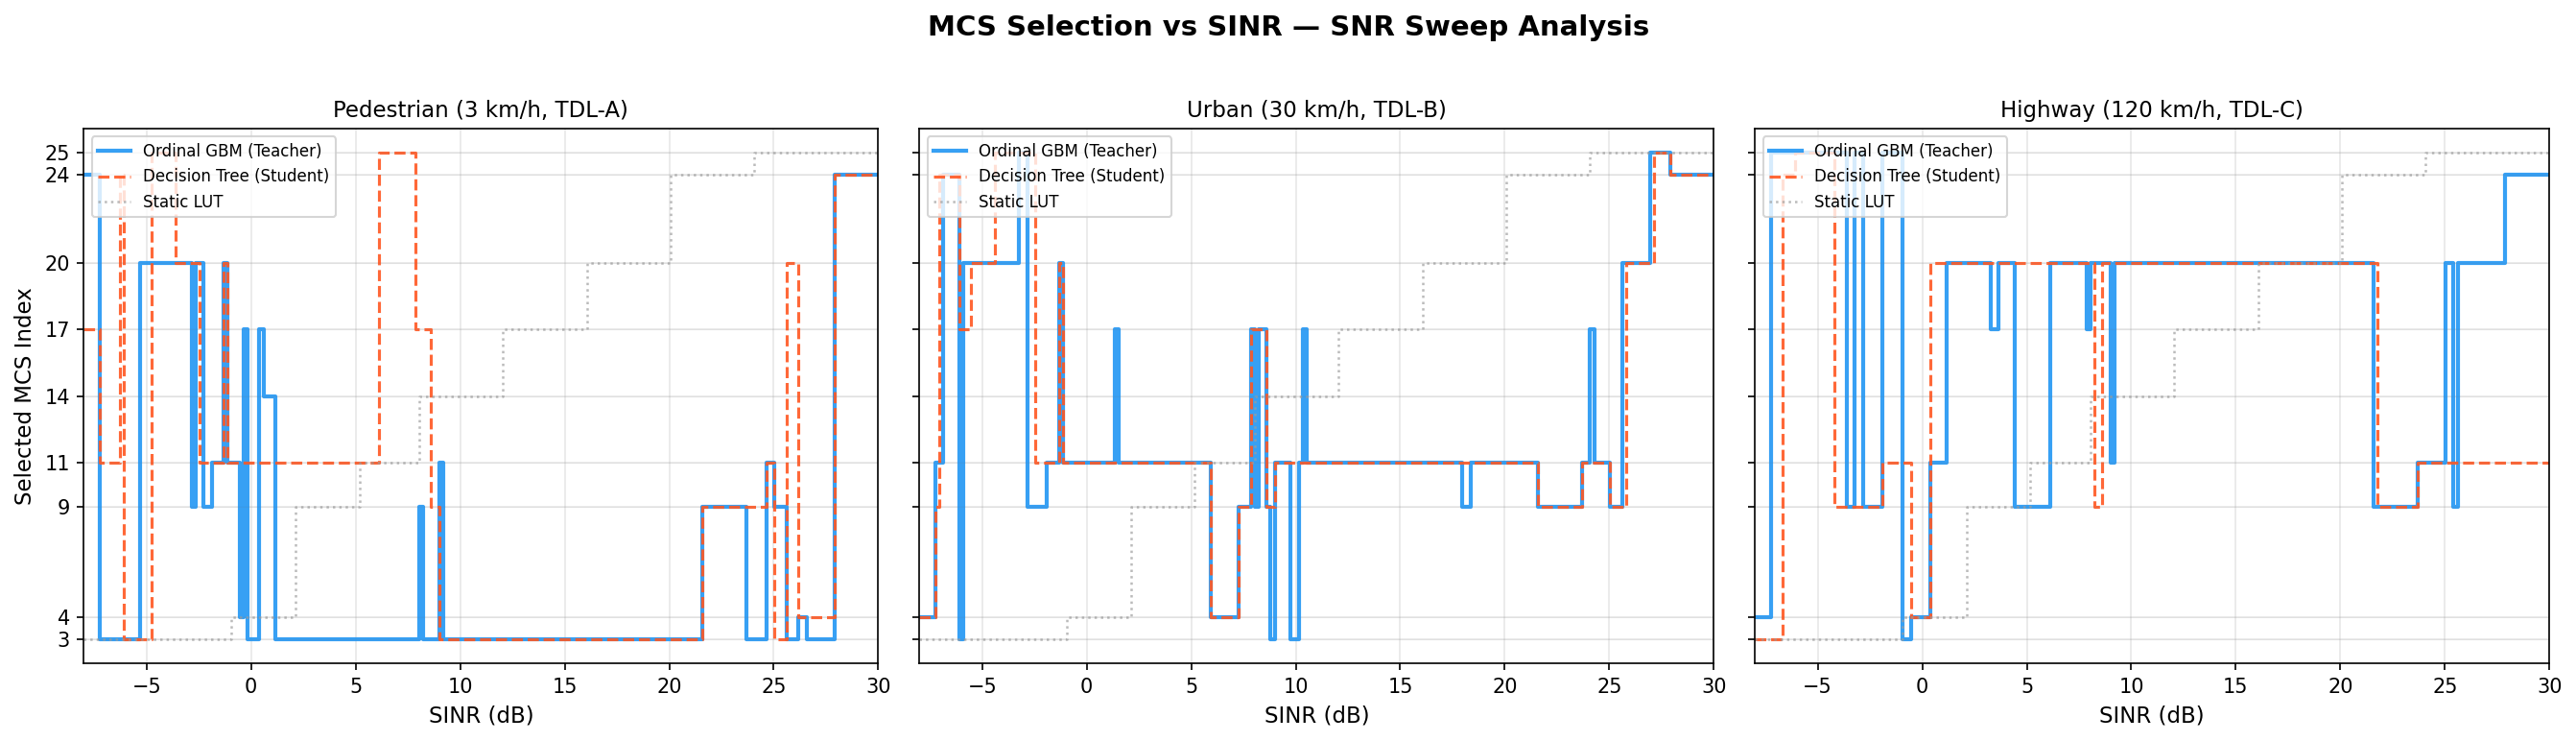
\includegraphics[width=0.48\textwidth]{results/snr_sweep_analysis.png}
    \caption{Zgodność destylacji (po lewej) oraz profil zależności MCS od SINR (po prawej).}
    \label{fig:distillation_snr}
\end{figure}

\subsection{Symulacja Zamkniętej Pętli}
Zasymulowano działanie algorytmów wraz ze sprzężeniem zwrotnym HARQ (ACK/NACK). Wyniki potwierdzają założenie o wyższości architektury hybrydowej. 

\begin{figure}[H]
    \centering
    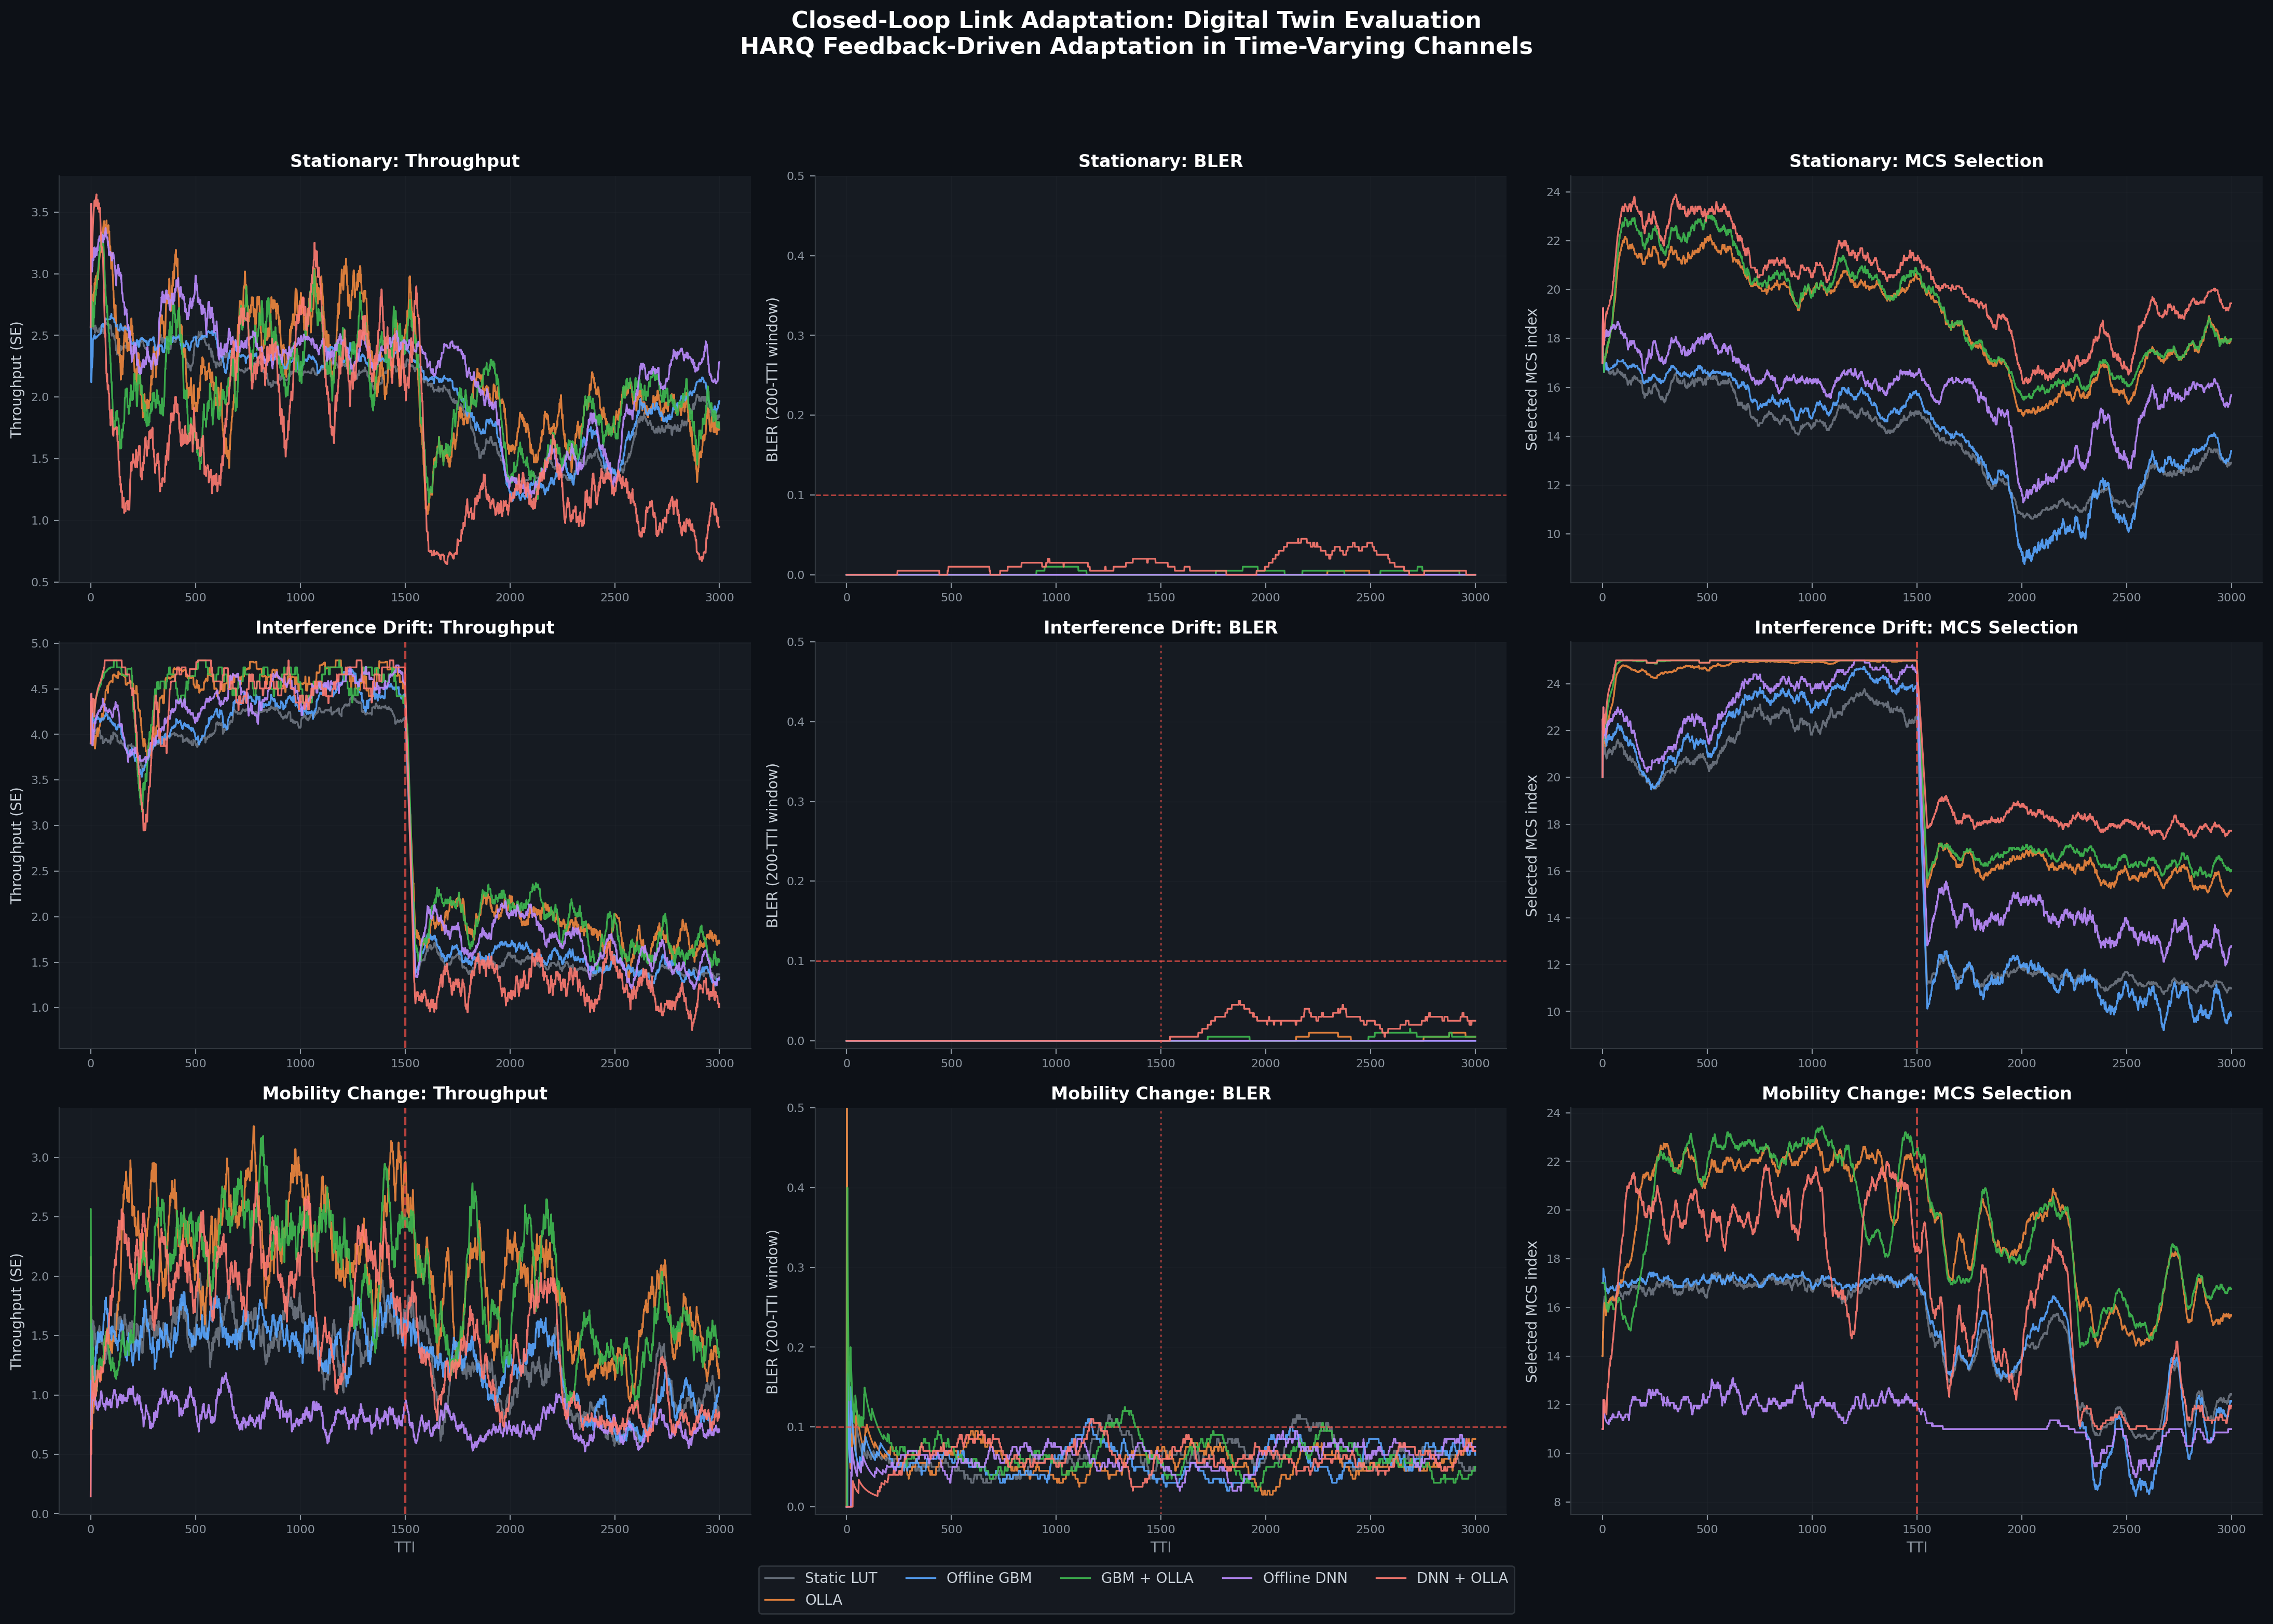
\includegraphics[width=0.8\textwidth]{results/online_la_results.png}
    \caption{Przebiegi zamkniętej pętli sprzężenia dla wybranych agentów.}
    \label{fig:online_simulation}
\end{figure}

W scenariuszu zmiennej prędkości (3 $\rightarrow$ 120 km/h), czysty mechanizm OLLA oraz połączenie GBM+OLLA utrzymują przepustowość na poziomie ok. 1.95-2.00 jedn. przy BLER na poziomie 5-6\%. System DNN+OLLA okazał się niestabilny w warunkach statycznych (generując BLER 1.2\%, co dyskwalifikuje go w usługach niezawodnych).

\subsection{Szybkość Działania (Benchmark C++)}
Wyeksportowane drzewo decyzyjne zostało przetestowane pod kątem wydajności w czystym C++ (flaga -O2). 
Test obejmujący milion wywołań wykazał średni czas predykcji na poziomie \textbf{84 nanosekund} (99. percentyl = 200 ns). Oznacza to, że algorytm pochłania zaledwie \textbf{0.008\%} dostępnego budżetu czasowego (1 ms), dowodząc pełnej gotowości do implementacji w systemach czasu rzeczywistego (RTOS).

\subsection{Testy na Żywo (srsRAN 5G NR)}
Finalnym etapem było wdrożenie zdestylowanego modelu C++ w kodzie źródłowym stacji bazowej (gNB) oprogramowania srsRAN Project. Testy przeprowadzono w sieci 5G SA z wykorzystaniem wirtualnego radia ZeroMQ oraz rdzenia Open5GS. 

\begin{figure}[H]
    \centering
    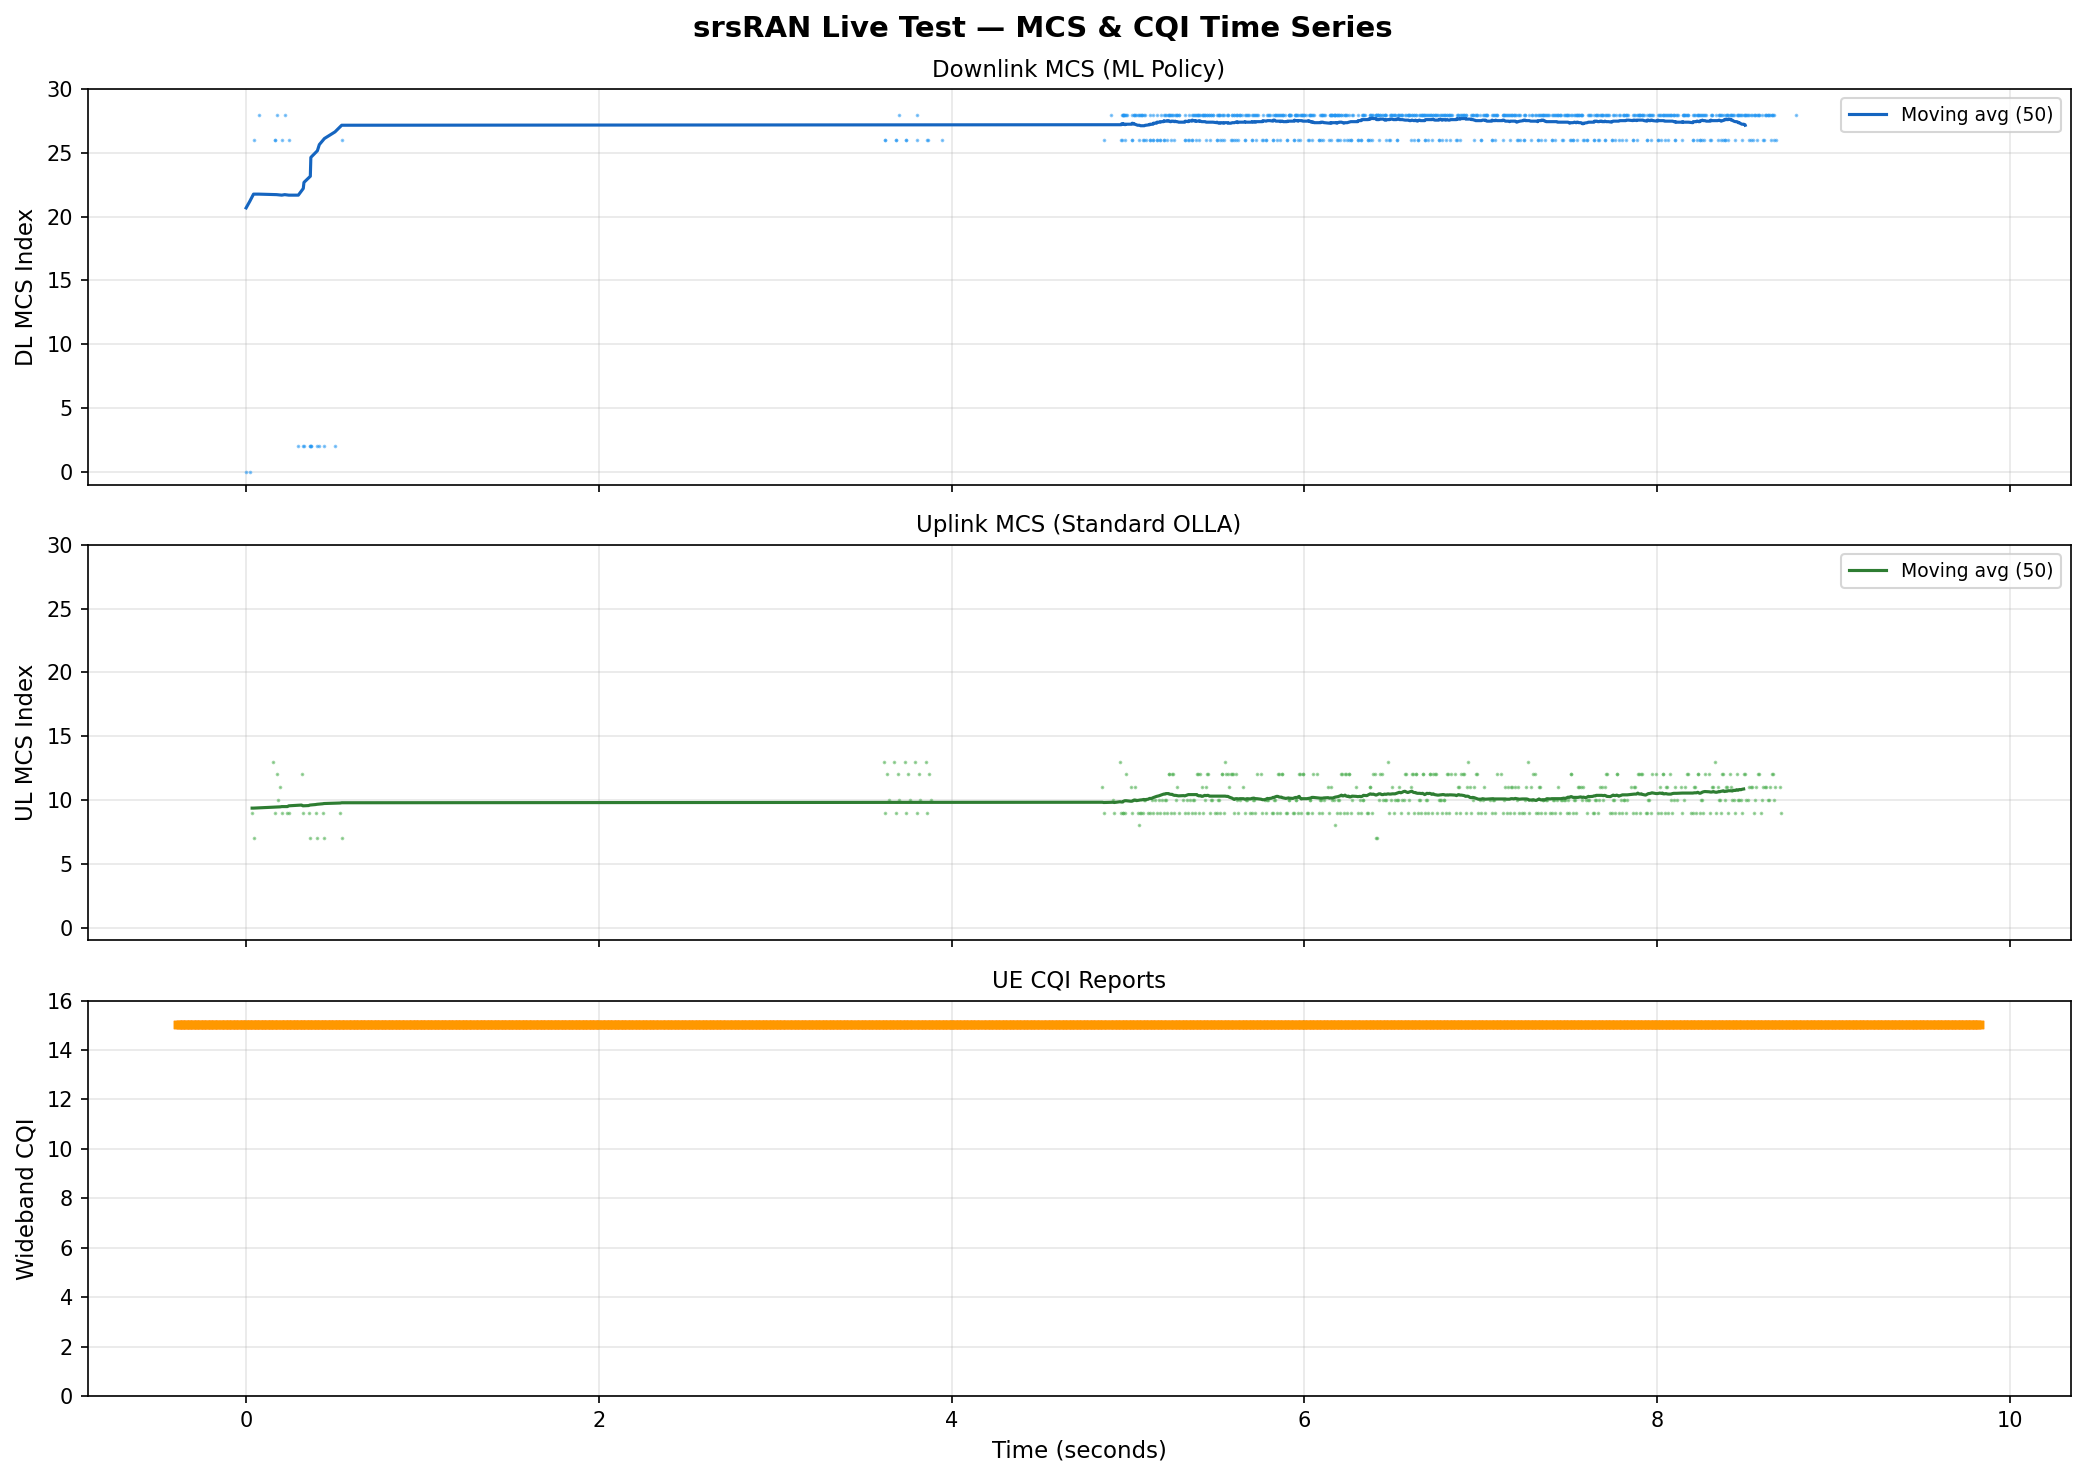
\includegraphics[width=1\textwidth]{results/srsran_mcs_timeseries.png}
    \caption{Przebieg czasowy dobieranego MCS przez stację bazową z wdrożonym modelem ML.}
    \label{fig:srsran_timeseries}
\end{figure}

Podczas testów przepustowości UDP zestawiono w pełni funkcjonalną sesję PDU (0\% utraty pakietów ICMP). Analiza logów warstwy PHY telefonu (srsUE) udowodniła aktywność modelu uczenia maszynowego: algorytm ustalał w łączu w dół wysokie wartości MCS (26-28), reagując na idealne warunki propagacyjne symulowanego kanału, co potwierdza histogram rozkładu predykcji.

\begin{figure}[H]
    \centering
    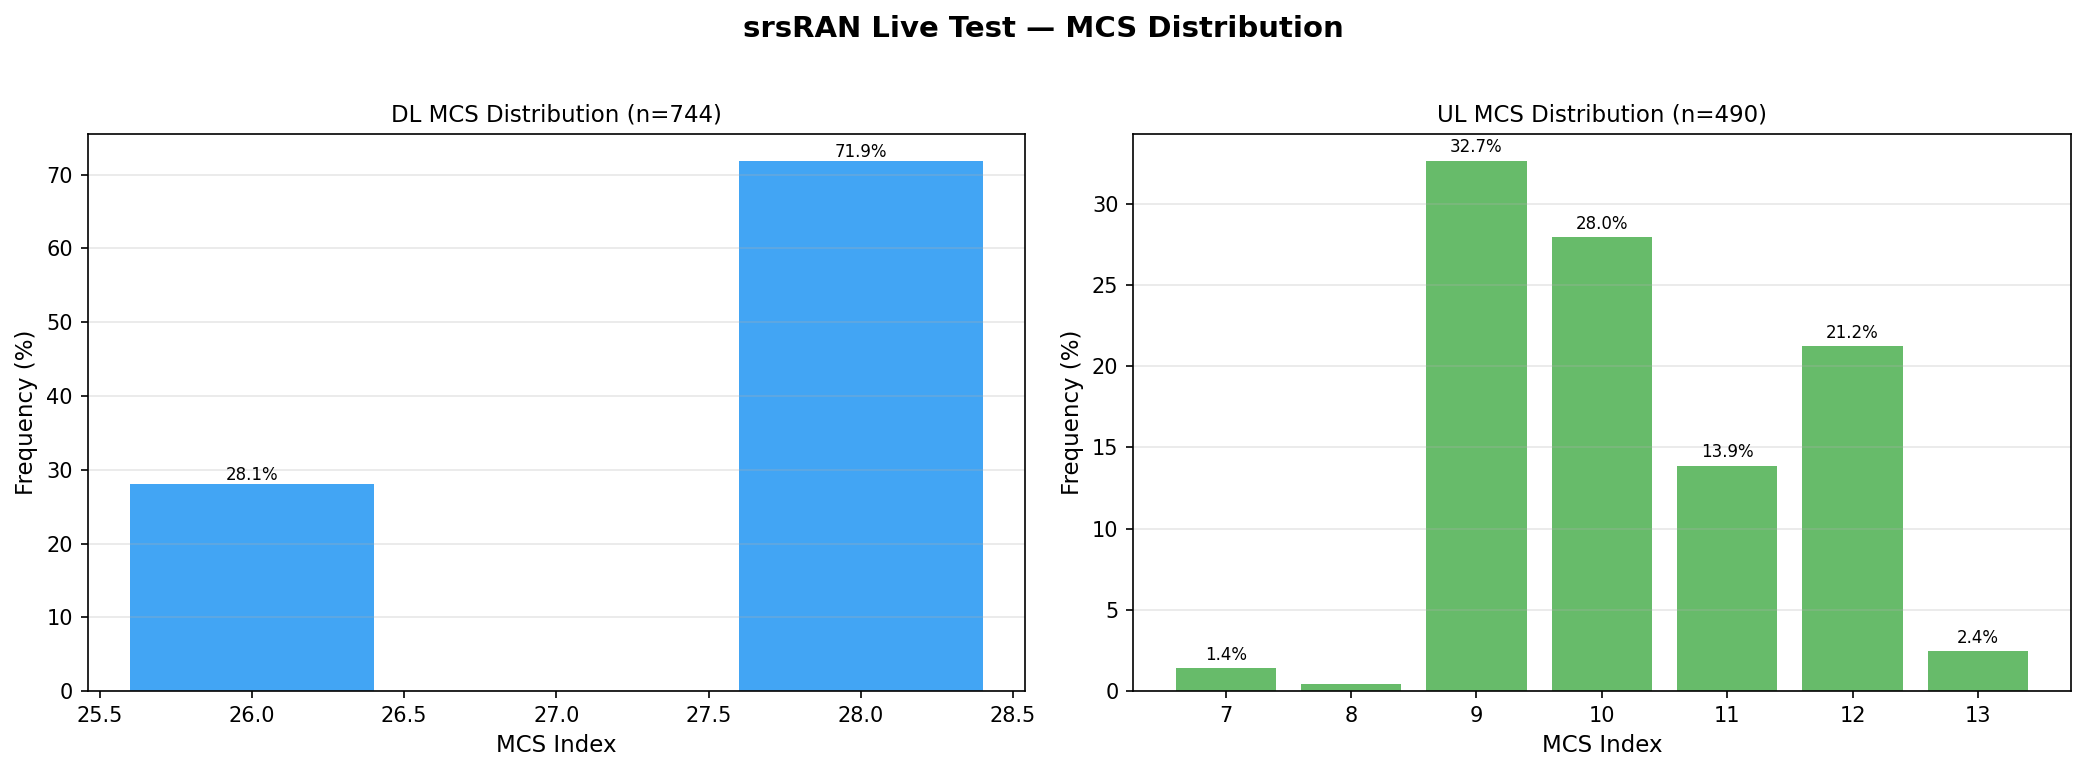
\includegraphics[width=0.8\textwidth]{results/srsran_mcs_distribution.png}
    \caption{Dystrybucja wybranych schematów MCS podczas testów w srsRAN.}
    \label{fig:srsran_dist}
\end{figure}

\section{Wnioski}
Zrealizowany projekt dowodzi praktycznej przydatności algorytmów uczenia maszynowego w systemach telekomunikacyjnych L2. Kluczem do sukcesu nie jest stosowanie najgłębszych sieci neuronowych, lecz zrozumienie domeny problemu (regresja porządkowa), fizyki (ograniczenia monotoniczne) oraz ograniczeń sprzętowych (destylacja wiedzy). Połączenie predykcji drzew decyzyjnych z reaktywną korekcją klasycznego pętli OLLA stanowi stabilne, profesjonalne rozwiązanie problemu adaptacji łącza.

\end{document}
